\documentclass[a4paper]{article}

\usepackage{graphicx}
\usepackage{amsmath,amssymb}
\usepackage{minted}
\usepackage{multirow}
\usepackage{float}
\usepackage{algorithm}
\usepackage{algpseudocode}
\usepackage{todonotes}
\usepackage{forest}
\usepackage{xstring}
\usepackage{xcolor}
\usepackage[most]{tcolorbox}
\usepackage{xparse}
\usepackage{natbib}
\usepackage{adjustbox}

\usetikzlibrary{graphs,graphdrawing}
\usegdlibrary{layered}

% for external graphviz
\input{/home/donkarlo/Dropbox/repo/nd_language_ai_project/src/nd_language_ai/formal/computer/programming/tex/latex/code_clips/external_graphviz.tex}

% for tags
\input{/home/donkarlo/Dropbox/repo/nd_language_ai_project/src/nd_language_ai/formal/computer/programming/tex/latex/part/control_sequence/kind/semtag/semtag.tex}

% for links
\input{/home/donkarlo/Dropbox/repo/nd_language_ai_project/src/nd_language_ai/formal/computer/programming/tex/latex/code_clips/seehere.tex}

% for nested lists and sections
\input{/home/donkarlo/Dropbox/repo/nd_language_ai_project/src/nd_language_ai/formal/computer/programming/tex/latex/code_clips/deep_structure.tex}

\title{}
\date{}
\author{Mohammad Rahmani}

\begin{document}
   \maketitle
   \seeherefooter{https://deutsch.lingolia.com/en/listening/b1/articles/sightseeing-tour-35151}
   \section{Transcription}
      Ich wohne in einem kleinen Ort, der an einer beliebten Wanderroute liegt. Im Sommer kommen Touristen aus dem In- und Ausland hierher. Oft sind sie sehr müde, weil sie so viele Kilometer mit dem Rucksack gewandert sind. Zum Glück haben wir einen Campingplatz oder mehrere Hotels, wo man übernachten kann.

      Weil unser Ort so schön ist, machen viele Wanderer hier ein paar Tage Pause, um sich umzusehen. Sie sind immer ganz begeistert und machen mit ihren Kameras unzählige Fotos.

      Mein Onkel ist Reiseleiter und führt oft Touristengruppen durch den Ort. Die Touren beginnen an der Touristeninformation, wo man auch Ansichtskarten und einen Stadtplan kaufen kann. Mein Onkel geht mit den Besuchern durch den mittelalterlichen Stadtkern, an einigen Denkmälern vorbei bis hin zum Schloss. Durch ein Fernglas zeigt er auch die Ruinen einer alten Burg in den Bergen. Wenn man dorthin wandern will, folgt man einfach den Wegweisern.
      \begin{figure}[H]
         \centering
         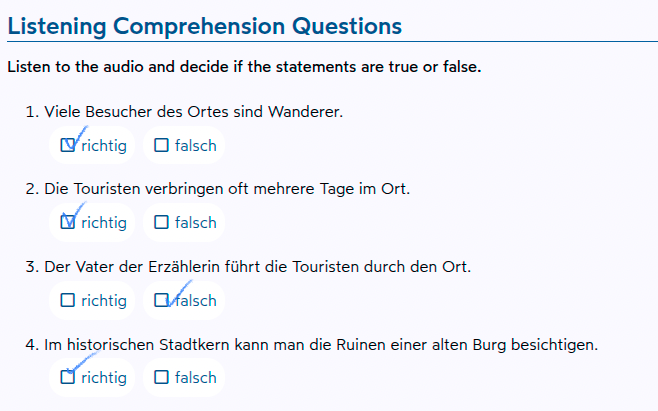
\includegraphics[width=0.9\textwidth]{img_0.png}
      \end{figure}


      \bibliographystyle{plainnat}
      \bibliography{/home/donkarlo/Dropbox/repo/nd_shared_research/bibliography/bibliography.bib}
\end{document}
